\chapter{Data Acquisition}
\label{ch:sp-daq}

%%% todo

% Assign candidate names to sections and solicit them to write notes and/or presentations.

% Start and maintain a list holding links to all relevant notes and presentations.

\fixme{\textbf{Authors:}

  See \url{https://wiki.dunescience.org/wiki/Technical_Design_Report}
  for general guidance. 

  While this chapter is still in outline, \textbf{check that it hits all
  the required points} some of which are:

  We are to describe a \textbf{baseline} or \textbf{process to
  decide a baseline}.

  \textbf{BE SUCCINCT} $TDR \approx IDR + 10\%$, goal is 50 pages for
  this chapter. 

  You are encouraged to produce \textbf{tech notes} with any
  supporting verbosity which may be referenced.

  State requirements and demonstrate how they are met, use
  standardized requirements table.

  Emphasize safety and professionalism (projectisms: cost, schedule,
  risks, interfaces).}

\metainfo{Some sections of this chapter must be written generically
  and without any reference to module-specific terms. They are marked
  with an orange ``fixme'' box. 
  Yellow info boxes like this one provide guidance for the content. 
  This guidance is not comprehensive so authors may provide additional
  information but retaining \textbf{conciseness} and \textbf{not
    repeating} info in other section is required.}

\section{Introduction}
\label{sec:fd-daq:introduction}
% \fixme{module-generic}

% \metainfo{A brief introduction to this chapter describing what will be
%   described.  This is \textbf{not} an overview of the DAQ itself.
%   Keep it brief. Do \textbf{not} write a conceptual overview here,
%   that is below, reference it. 
%   Do \textbf{not} use module-specific language but \textbf{do}
%   describe how commonalities are described in text shared by both
%   SP/DP volumes and specialized sections appear only in their
%   respective volume. 
%   \textbf{Do} describe the lexicographical convention used to demark
%   shared sections (this needs coordination with other chapters in the
%   same boat).}

The design of the \dword{dune} \dword{fd} \dfirst{daq} system is described in this chapter.  The DAQ services all \dword{fd} \dwords{detmodule}.  Most  aspects of the design are identical across the different \dwords{detmodule} and they are described in sections below which are reproduced verbatim in this \dword{daq} chapter in each \dword{detmodule} TDR volume.  A minority portion of the DAQ design that must be tailored to meet module-specific requirements are documented in sections below which are unique to each \dword{detmodule} TDR volume.  These sections are identified simply by their module-specific language.

The sections below begin with the requirements for and interfaces between DAQ and other DUNE systems.  A section comparing the \dword{protodune} experiment with DUNE is given to highlight important information learned from that prototype and what still must be understood.  The subsequent section describes the design itself.  The chapter finishes with giving details on project management issues such as production, installation, cost, schedule, safety, and other items.

\section{Requirements}
\label{sec:fd-daq:requirements}
\fixme{module-generic}

\metainfo{One sentence introducing the contents of this section.}

\subsection{Specifications}
\label{sec:sd-daq:specifications}
\fixme{single-phase module}


\metainfo{Include rows of top-level requirements table (``Schmitz''
  table) here. 
  Augment that with any additional requirements of our determining. 
  Eg: accept data from detector electronics, perform reduction to
  satisfy output rate limit, allow for cross-module triggering,
  collect beam activity with XX\%, SNB requirements, noise level,
  total thermal and space envelop, etc....}

\metainfo{Include message passing requirements and domains.}

\subsection{Design Philosophy}

\metainfo{Describe how the design addresses the requirements.}

\subsection{Parameters}
\label{sec:sp-daq:parameters}
\fixme{single-phase module}

\metainfo{Include a table which lists all important parameters driving
  the design.  Sampling rate and resolution, channel count}


\section{Interfaces}
\label{sec:sp-daq:interfaces}
\metainfo{Include interface summary and table here.}
\subsection{TPC Cold Electronics}
\metainfo{Data reception physical and logical, configuration information delivery.}
\subsection{PDS Readout System}
\metainfo{Data reception physical and logical, configuration information delivery.}
\subsection{Computing}
\metainfo{Buffer disk. 
  Agreement on sysadmin support and computer procurement, ssh gateways, non data networks. 
  Address reference how the data model described above is acceptable.}
\subsection{CISC}
\label{sec:sp-daq:interfaces-cisc}
\subsection{Calibration}
\subsection{Timing}
\metainfo{Note, this is an ``outgoing'' interface from DAQ's Timing System to various others. 
  Instead of making this section explicit we may instead disperse Timing System interface information among the other Interface sections where appropriate.}

\section{ProtoDUNE and DUNE Comparison}

\metainfo{Here we write what similarities and differences there are between ProtoDUNE and DUNE DAQ designs.}

\subsection{Detector Readout Hardware}

\metainfo{Compare and contrast design elements related to the detector readout hardware.}

\subsubsection{RCE}

\subsubsection{FELIX}

\subsection{Backend Event Building}

\subsection{Other}

\section{DAQ Design}
\label{sec:fd-daq:design}
% \fixme{module-generic}

% \metainfo{One sentence to introduce the section. 
%   Listing the subsections and describing which are generic and which
%   are X-phase specific.}

This section describes the DAQ design. 
It begins with a conceptual overview followed by sections giving the design of the DAQ subsystems. 
First come the \dword{ipc} and \dword{ccm} subsystems.
Next is the \dword{fe} data receiver and data handling and processing subsystems.
Then, the subsystems for data selection and the DAQ back-end are described Finally, the timing subsystem is presented and this section finishes with plans for design validation and development.


The following descriptions of the design are kept brief due to page limitations. 
More details are provided as technical notes as listed in Table~\ref{tab:fd-daq:tech-notes}.

\begin{dunetable}{|p{0.7\textwidth}|p{0.2\textwidth}|}{tab:fd-daq:tech-notes}{Summary of relevant and detailed DAQ technical notes.}
  Title & References \\
  DUNE Far Detector Data Volumes & \citedocdb{9240}\\
  The DAQ for the single phase DUNE Prototype at CERN & \citedocdb{8708}\\
  A System for Communication Between DAQ Elements & \citedocdb{10482}\\
  Data Selection for DUNE Beam and Atmospheric Events & \citedocdb{11215}\\
  Data orchestrator and event building for DUNE FD DAQ & t.b.d. \\
  DUNE Run Control, Configuration \& Monitoring (CCM) & t.b.d. \\
  DUNE DAQ Readout & t.b.d. \\
\end{dunetable}



\subsection{Overview}
\label{sec:fd-daq:design-overview}
%\fixme{module-generic}

\begin{dunefigure}{fig:daq-conceptual-overview}{DAQ Conceptual
    Subsystem Overview.  See text for description.}
  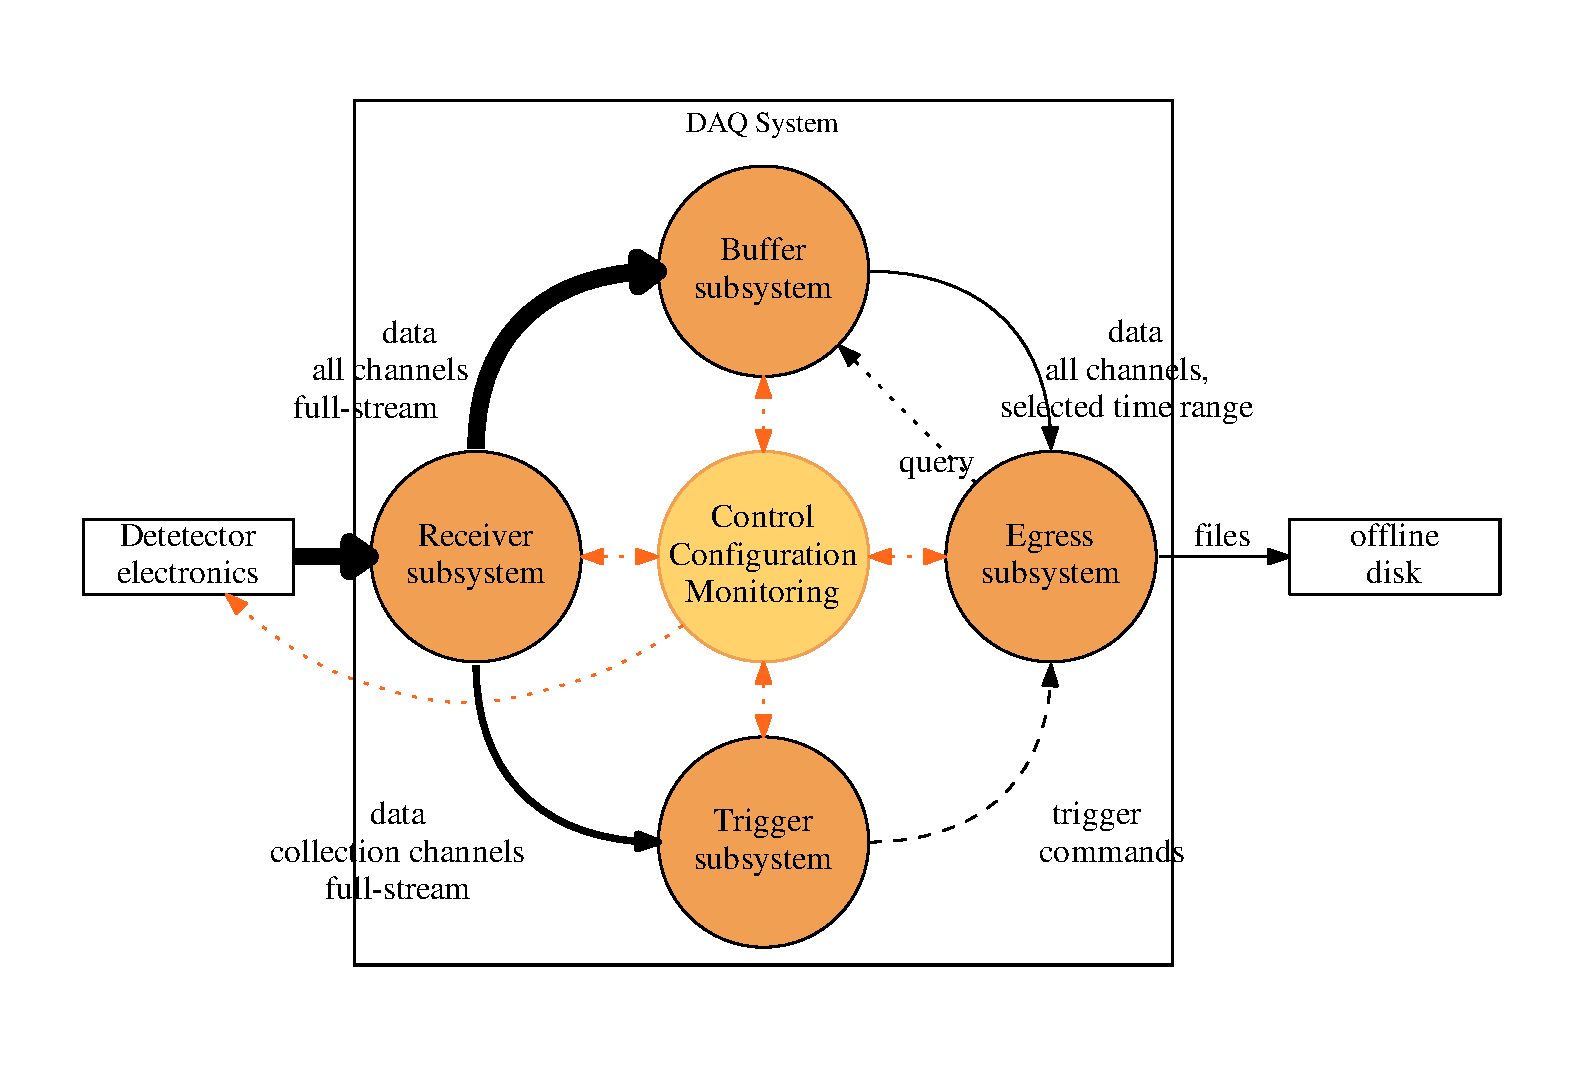
\includegraphics[width=0.8\textwidth]{daq-toplevel-conceptual.pdf}
\end{dunefigure}

% \metainfo{This is the \textbf{only} place to describe the conceptual
%   overview. 
%   Do \textbf{not} repeat this info in sections below. 
%   \textbf{Do} use \textbf{module-neutral} terms.
%   \textbf{Do} describe major interface between each subsystem (the edges between the circles in Fig~\ref{fig:daq-conceptual-overview}).
%   \textbf{Do} mention that concrete systems span portions of the
%   conceptual subsystems and how the following subsections are defined
%   along these concrete deliverable lines.}

An illustration of the conceptual parts which make up the DUNE FD DAQ is given in Fig.~\ref{fig:daq-conceptual-overview}. 
It applies to all \dword{fd} modules. 
The box in the illustration indicates the overall scope of the DAQ.
Each of the various concrete hardware and software subsystems describe later in this section provide a portion of one or more of the conceptual subsystems represented by the circles in the figure.
Approximately following the data flow through the DAQ, the concept starts with receiving input via optical fibers from the detector electronics (see Section~\ref{sec:fd-daq:design-felix}). 
The flow then bifurcates. 
The entirety of the input flow is buffered for a period of time sufficient to satisfy triggering and readout requirements (see Section~\ref{sec:sp-daq:design-fe-processing}). 
The second flow need contain only data that is to be used to form a \dword{trigdecision} (see Section~\ref{sec:sp-daq:design-selection-algs}).
The information in that decision is used by the egress subsystem to query back to the appropriate buffers and thus retrieve selected data (see Section~\ref{sec:fd-daq:design-backend}).
The results are aggregated and saved to files on nonvolatile storage media at which point custody is transferred to offline responsibility.
This is all orchestrated by the \dword{ccm} subsystem (Section~\ref{sec:fd-daq:design-run-control}) shown in the center of the figure.   The various information flows, represented by the arrows of the figure, ride on the \dword{ipc} subsystems (Section~\ref{sec:fd-daq:design-messages}). 

\metainfo{Include components summary and table here.  Need guidance on what is wanted.}

\fixme{Where will we describe partitions?}
As described more in Section~\ref{sec:fd-daq:partitions}, this conceptual picture is implemented in terms of a number of \dwords{daqpart} or instances. 
The primary set of partitions will exist underground in the \dword{cuc} in order to service the \dword{fd} modules. 
As described more in Section~\ref{sec:sp-daq:production} the DAQ will connect to and begin servicing portions of a \dword{fd} module after they are installed and commissioned. 
There will also be a DAQ presence in the \dword{itf} to support the work there during detector construction.
% \metainfo{Include physical location description}




\metainfo{For the remaining design sections: do not include directly validation info but rather place this information in section~\ref{sec:sp-daq:design-validation} and make references.}
  



\subsection{Inter-process Communication}
\label{sec:fd-daq:design-messages}
\fixme{module-generic}

The DAQ must transfer data of various schema, latency and throughput. 
For the most part these transfers must be reliable in that once data is sent it is received if the recipient is accessible on the network and operational. 
As detailed in Section~\ref{sec:sp-daq:design-selection-algs}, one particularly critical element is the unit which makes the pinnacle trigger decision. 
It shall be developed to support redundancy. 
This will largely be satisfied by having IPC communication units follow the \dword{pubsub}.


Choices of IPC systems impact performance, functionality, development and support costs among others. 
Some subsystem solutions bring their own IPC system while developers of the required novel systems must select a suitable IPC system. 
The choice is one which must balance trade-offs. 
The development philosophy is to minimize the number of distinct IPC systems while embracing existing ones which accompany high quality solutions for implementing subsystems.

In general, an IPC domain covers IPC units which have support for the associated IPC system. 
The DUNE FD DAQ shall select and develop a \textit{lingua franca} IPC system to be used for inter-domain IPC and as a candidate for direct use in any required novel development.  Any domain that does not naively support the \textit{lingua franca} IPC shall have a proxy or gateway unit developed that translates between the two.

An example of a subsystem that shall support the IPC \textit{lingua franca} is the hierarchical trigger processing system provided by the data selection (Section~\ref{sec:sp-daq:design-selection-algs}. 
An example of a subsystem providing its own IPC domain is artDAQ which shall provide the heart of the egress system (Section~\ref{sec:fd-daq:design-backend}).
The DAQ shall also interface with external domains. 
For example, a two way exchange of information between DAQ and \dword{cisc} shall be developed as described in Section~\ref{sec:sp-daq:interfaces-cisc}.

\fixme{Shall we name ZeroMQ specifically as the basis for the \textit{lingua franca} IPC?}

% \metainfo{Describe the domains requiring message passing.  A domain means parts that shall share the same message passing infrastructure.  Eg, the hierarchical trigger system is one.  The transfer of data between artDAQ nodes is another.  Run control, monitoring and logging is a third.  Some MP domains will exist in other consortia and must interface with DAQ MP domains.  Each internal or external interface must be at least listed.   Describe how effort will be conserved by minimizing the number of distinct domains to the extent it makes sense.  Some examples: two-way comms with CISC (CISC tells DAQ of HV it shut down, DAQ tells CISC about hardware health, DAQ process health, statistics on things like per-unit trigger rates), handling laser triggers (eg, want laser to only fire in between beam spills).}

% \metainfo{We may not be ready to give concrete designs for every domain.  Where this is the case, we must describe a plan for determining the IPC system for each domain.}

%\metainfo{IPC must support redundant paths for trigger information, especially at the MLT level and above, to assure robustness.}


\subsection{Control, Configuration and Monitoring}
\label{sec:fd-daq:design-run-control}
\fixme{module-generic}

\metainfo{Describe run control and DAQ operation monitoring. 
  How it makes use of the Message Passing System. 
  What is an ``epoch''.
  How Epoch Change Requests lead to zero down time reconfiguration. 
  Public key based ``iron'' authentication between run control processes and the controlled processes. 
  Describe how RC will configure partitioning, initiate reconfiguration, handle ``run'' changes, node discovery, configuration, logging, startup, shutdown and failures are handled. Describe how RC will support detector electronics configuration.}

The \dword{ccm} subsystem encompasses all the software that is needed to control, configure and monitor the rest of the DAQ and to some extent its own subsystem. 
It acts as a glue for the different DAQ components allowing them to be treated and managed as a coherent system, while not dealing directly with the primary transport of physics data, nor with their selection, nor with the orchestration of the data movement. 
A pictorial view of the central role of the \dword{ccm} within the complete DAQ system was shown in Figure~\ref{fig:daq-conceptual-overview}.

The \dword{ccm} is composed of three main sub-systems, the Control, the Configuration and the Monitoring, each with a well-defined role:
\begin{itemize}
\item The Control sub-system is in charge of managing the lifetime of the DAQ software processes, ensuring the respect of access and resource management policies; it is responsible for distributing commands to the different DAQ components and of detecting and handling errors; last, but not least, it offers a user interface allowing the operators and experts to act on the different DAQ system instances (Partitions).
\item The Configuration sub-system consists of a database, a historic view of configurations used for data taking, a unique run number service, a configuration editor allowing experts to define the parameters needed for all components of the DAQ, and a data access layer allowing DAQ applications to retrieve relevant configuration parameters.
\item The Monitoring sub-system provides the mechanisms for applications to publish and subscribe to information, messages and a sub-set of event data, for the purpose of monitoring and diagnosing the behavior of the DAQ system as well as the quality of the physics data.
  In addition, it offers the possibility of archiving information, messages and histograms, thus allowing to keep a history of the system behavior and to carry out a posteriori system analysis when needed.
\end{itemize}

The three \dword{ccm} sub-systems interact and operate together to guarantee efficient data taking. As an example, as shown in Figure~\ref{fig:daq-ccm-subsys}, the Control sub-system relies on the Configuration to know which components participate the a DAQ instance, which policies to apply for resource management and error handling and uses the Monitoring in order to retrieve the status of DAQ components and detect any anomalies.

It shall be noted that, while the CCM system is instrumental to the definition of the data taking conditions, the conditions database, as well as the definition of which conditions are important for offline analysis are not part of the CCM. The CCM will provide the required information on request.

\begin{dunefigure}{fig:daq-ccm-subsys}{Main interaction between the three CCM sub-systems.}
  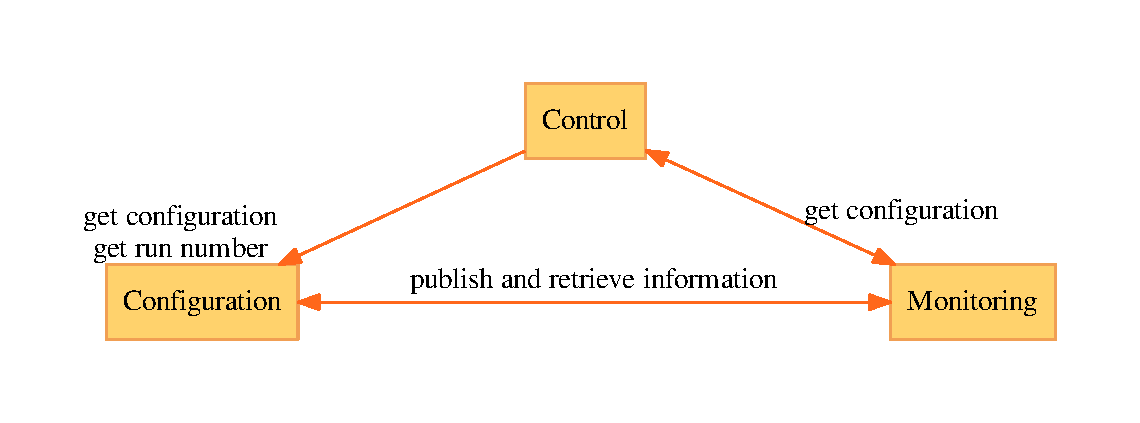
\includegraphics[width=0.8\textwidth]{daq-ccm-subsys.pdf}
\end{dunefigure}

\fixme{There are still requirements and then detailed subsections on the three CCMs subsystems to consider adding.}



\subsection{Detector Data Receiver}
\label{sec:fd-daq:design-felix}
\fixme{module-generic}

\metainfo{Describe how FELIX hardware defines an interface which common to all modules.  Describe how the hardware may handle UDP or other prototocols including bidirectional communication.  Describe how FELIX can be scaled to accept data across a spectrum in order from large to small data rate: the full SP data from the WIBs, full compressed data from the DP, trigger primitive stream from FPGA based units placed between WIBs and FELIX.}


\ifdp
\subsubsection{DP data ingest via UDP}
\label{sec:dp-daq:design-udp-ingest}
\fixme{dual-phase module, move to DP-DAQ chapter eventually}
\metainfo{This is a DP section and will be only in the DP volume. 
  It should describe the ``Bump On Wire'' from the IDR unless we can
  come up with any new/better ideas.}
\metainfo{Include full hardware scope starting at fibers from CE and
  ending at the output of trigger processors and the interface between
  buffer and the Data Selector.
  Describe the per-APA multiplicity of computers, CPU cores, host
  system RAM, host system storage, FELIX boards, DPM components (RAM,
  SSD). 
  Include thermal estimates itemized by components.}  
\fi

\subsection{Front-end Data Handling and Processing}
\label{sec:sp-daq:design-fe-processing}

\metainfo{This section describes four functional blocks: (1) 10s RAM buffer (minimum), (2) non-volatile SNB buffer for 30s of data once per month (minimum), (3) hardware for the production of trigger primitive including any data formatting and DPS filtering and (4) compression of selected data.  Note, actual algorithms for trigger primitives are described in Section~\ref{sec:sp-daq:design-selection-algs}.}

\metainfo{One or two sentences that positions the two processing
  patterns (FEDHP either before or after FELIX) in this section as options. 
  Say that the ``FPGA before FELIX'' option is used for ``baseline costing''.}

\metainfo{Include a table with one row for each known compression factor: protoDUNE RCE and FELIX, MicroBooNE before and after noise filter (see docdb), 35t, protoDUNE data after ADC stuck code mitigation or avoidance, simulations.  One column of this table shall give a brief comment of how it applies to DUNE including any caveats or reasons for over/under estimation.}

% \subsubsection{FELIX+FPGA}
\subsubsection{Upstream FPGA and Firmware}
\label{sec:sp-daq:design-felix-fpga}
\fixme{single-phase module}

\metainfo{Include full hardware scope starting at fibers from CE and
  ending at the output of trigger processors and the interface between
  buffer and the Data Selector.
  Describe the per-APA multiplicity of computers, CPU cores, host
  system RAM, host system storage, FELIX boards, DPM components (RAM,
  SSD). 
  Include thermal estimates itemized by components.}

% \subsubsection{FELIX+CPU}
\subsubsection{Downstream CPU and Software}
\label{sec:sp-daq:design-felix-cpu}
\fixme{single-phase module}

\metainfo{Include full hardware scope starting at fibers from CE and
  ending at the output of trigger processors and the interface between
  buffer and the Data Selector. 
  Describe the per-APA multiplicity of computers, CPU cores, host
  system RAM, SSD and FELIX boards. 
  Include thermal estimates itemized by components.}


\subsubsection{Photon Detection System Interface}

\metainfo{Some motivations for using light to trigger. 
  (1) want to understand PDS so want to trigger on just the PDS. 
  (2) background to SNB for which PDS trigger primitives may eliminate. 
  (3) possibly must rely on light only for SNB triggering, eg if noise is out of control. 
  Some to all of these should be included.}

\metainfo{Possibly want to \SI{1}{\micro\second} packet for every time a 1-PE threshold is crossed. 
  PDS is still understanding what they may send. 
  DAQ needs to be in control of the trigger forming.}

\subsubsection{DP TPC FE issues}

\fixme{dual-phase module}

\metainfo{This is similar to SP except for the need to decompress before any trigger primitive processing.  Decompression can potentially happen on FELIX FPGA or on CPU.  There shall be a table or description of the amount of processing required.}

\subsubsection{DP SP Issues}
\fixme{dual-phase module}




\subsection{Data Selection}
\label{sec:sp-daq:design-selection-algs}
\fixme{single-phase module}

\fixme{There are many studies which could go into this section. Some of this may very likely be moved into one or more tech notes and referenced.}


Data Selection must make the decision about what data will be
transferred to the Backend Subsystem. 
It does by providing the core payload software which runs in message
passing nodes. 
In particular it provides the trigger primitive, candidate and
command hierarchy.

\metainfo{One sentence that briefly describes the ``bow tie''
  hierarchy: primitive, candidate, command, query. 
  Do not repeat too much what is in the design overview. 
}


\subsubsection{Trigger Primitives}
\label{sec:sp-daq:design-trigger-primitives}
\fixme{single-phase module}

\fixme{Trigger primitive algorithms run inside of the hardware of \ref{sec:sp-daq:design-fe-processing} but conceptually are more intimate with the Data Selection.  That section should reference this section.}

\metainfo{Describe what they are, how they are formed, storage size on disk, message schema. 
  This section describes algorithms with references to where those algorithms may run (FPGA firmware or CPU software)} \metainfo{Reference the section that provides validation.}


\metainfo{Include plot and discussion of DUNE trigger primitive rate in protoDUNE. 
  The fact that this includes many more cosmics will not matter much as the rate is expected to be dominated by Ar39. 
  Phil has this already but the LAr purity is not yet high enough to see Ar39 across the whole drift distance.}

\subsection{Back-end System}
\label{sec:fd-daq:design-backend}
\fixme{module-generic}

\metainfo{This subsystem starts with receiving trigger commands from MTL, based on their content it queries Data Selectors on all front end computers, forms events, writes files to offline buffer disk. 
  It may perform ``offline'' type processing along the way.}


\subsubsection{Event builder}
\label{sec:fd-daq:design-event-builder}
\fixme{module-generic}

\metainfo{Explain artDAQ, handling of trigger commands by asynchronous, parallel queries to front end Data Selector (but take care not to duplicate between here and in the overview).}

\subsubsection{L2 Data Reduction}

\subsubsection{Data Quality Monitoring}

\subsubsection{Data Model}
\label{sec:fd-daq:design-data-model}
\fixme{module-generic}

\metainfo{Describe the data model. 
  This isn't a strict schema just things like how various parts of the
  detector readout map to files, etc.}

\subsubsection{Output Buffer}

\metainfo{Describe the output buffer system, how it's shared with offline, data hand-off prototocols.  Responsibility scope (eg, who handles transfer to FNAL).}

\subsection{Timing Distribution}
\label{sec:sp-daq:design-timing}
\fixme{single-phase module}
\fixme{Is it indeed still single-phase specific?}

\metainfo{Hardware, consumers, links.}

\subsection{Design Validation and Development Plan}
\label{sec:sp-daq:design-validation}
\fixme{single-phase module}

\metainfo{One sentence to describe our validation strategy: exploit
  ProtoDUNE, use simulation and develope vertical slice tests. 
  Put each validation study (performed or future) in a subsubsection
  and describe either \textbf{how it justifies a decision} or
  \textbf{how its outcome will be used to make a decision in the
    future}.}

\subsubsection{FELIX Throughput Demonstration at ProtoDUNE-SP}
\label{sec:sp-daq:validation-pdune-felix}
\fixme{single-phase module}

\metainfo{Describe how the FELIX DAQ at ProtoDUNE-SP demonstrates a
  FELIX+CPU approach. 
  Describe the elements that are same or similar (full-rate to host
  RAM buffer) and different (higher-rate but external trigger).}


\subsubsection{RCE Throughput Demonstration at ProtoDUNE-SP}
\label{sec:sp-daq:validation-pdune-rce}
\fixme{single-phase module}

\metainfo{Describe how RCE DAQ at ProtoDUNE-SP demonstrates an FPGA
  approach with DUNE.}

\subsubsection{Trigger Primitives in Software}
\label{sec:sp-daq:validation-software-trigger-primitives}
\fixme{single-phase module}
 
\metainfo{Succinctly describe algorithm, include physics and computing
  performance numbers.}

\subsubsection{Trigger Primitives in Firmware}
\label{sec:sp-daq:validation-firmware-trigger-primitives}
\fixme{single-phase module}

\metainfo{Succinctly describe algorithm, include physics and computing
  performance numbers.}

\subsubsection{Vertical Slice Demonstrations}
\label{sec:sp-daq:validation-demonstrators}
\fixme{single-phase module}

\metainfo{Describe VST demonstrators and why we must build them.}

\subsubsection{Prototype Message Passing System}
\label{sec:fd-daq:validation-demonstrators}
\fixme{module-generic}

\metainfo{This is actually module-generic. 
  Very briefly describe the prototype message passing. 
  This will mostly refer to a tech note.}

\subsubsection{Another validation....}
\fixme{write me, as needed}

\section{Production, Assembly, Installation and Integration}
\label{sec:sp-daq:production}

\metainfo{Describe how hardware, firmware and software will produced. }


\metainfo{Describe how we get stuff in place underground (and in the
  ITF), how we will put it all together and make sure it works. 
  What can we do to minimize the effort needed underground both in
  terms of physical work but also in working out the bugs both in
  individual processes and in emergent behavior of the system as a
  whole?}

\subsection{Computing Hardware}

\subsection{Custom Hardware Fabrication}

\subsection{Software and Firmware Development}
\metainfo{Processes and practices.}

\subsection{ITF}

\section{Cost, Schedule, Safety and Risk Summary}
\label{sec:sp-daq:cost}
\metainfo{
Include cost summary and table here.
Include schedule summary and table here.
Include risk summary and table here.}

